\xiti
\begin{xiaotis}
\begin{enhancedline}

\xiaoti{求证:顺次连结正多边形各边中点所得的多边形是正多边形。}

\xiaoti{求证:正五边形的对角线相等。}

\xiaoti{求证:如果一个多边形有一个外接圆和一个内切圆,并且这两个圆是同心圆,那么这个多边形是正多边形。}

\xiaoti{已知: $AB$ 是 $\yuan\,O$ 的内接正六边形的一边,
    $AD$ 是 $\yuan\,O$ 的内接正十边形的一边,点 $D$ 在 $\yuanhu{AB}$ 上。
    求证: $DB$ 是 $\yuan\,O$ 的内接正十五边形的一边。
}

\xiaoti{求证:两个同边数的正多边形周长的比等于它们的外接圆直径的比。}

\xiaoti{在某个圆形盖板上钻 16 个等距离的小圆孔,使孔心和盖板中心的距离为 240 mm。
    求相邻两孔中心的距离(精确到 0.1 mm)。
}

\xiaoti{要用圆形铁片截出边长为 $a$ 的正方形铁片,选用的圆铁片的直径最小要多长?}

\xiaoti{如图,正六边形的螺帽的边长 $a = 12$ mm,这个搬手的开口 $b$ 最小应是多少?}

\begin{figure}[htbp]
    \centering
    \begin{minipage}[b]{7cm}
        \centering
        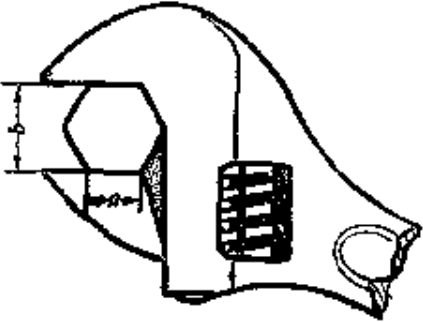
\includegraphics[width=5cm]{../pic/czjh2-ch7-xiti27-08.png}
        \caption*{(第 8 题)}
    \end{minipage}
    \begin{minipage}[b]{7cm}
        \centering
        \begin{tikzpicture}[scale=.7]
    \pgfmathsetmacro{\r}{0.2}

    % 设小圆的圆心为 O, OD 垂直于 O_1O_2, 垂足为 D。
    % 则,在直角三角形 DOO_1
    % OO1 = R + r
    % 因为:DO_1O = 30 度,所以, OD = OO1/2 = (R + r)/2
    %   R^ + [(R + r)/2]^2 = (R + r)^2
    % 化简得
    %   R^2 - 6Rr - 3r^2 = 0
    % 代入 r = 0.2 得
    %   R = 1.29
    \pgfmathsetmacro{\R}{1.29}

    \tkzDefPoints{0/0/O}
    \tkzDefPoint(210:\R+\r){O_1}
    \tkzDefPoint(330:\R+\r){O_2}
    \tkzDefPoint(90:\R+\r){O_3}

    \tkzDefCircle[R](O,\r)  \tkzGetPoint{o}
    \tkzDrawCircle[very thick](O, o)
    \foreach \n in {1,2,3} {
        \tkzDefCircle[R](O_\n,\R)  \tkzGetPoint{o_\n}
        \tkzDrawCircle[very thick](O_\n, o_\n)
    }
    \tkzDrawPolygon[dashed](O_1,O_2,O_3)
    \tkzDrawSegments[dashed](O,O_1)

    \tkzLabelPoints[left](O_1)
    \tkzLabelPoints[right](O_2)
    \tkzLabelPoints[above](O_3)
\end{tikzpicture}


        \caption*{(第 11 题)}
    \end{minipage}
\end{figure}

\xiaoti{已知圆内接正 $n$ 边形的边长为 $a$。 求同圆外切正 $n$ 边形的边长(用三角函数表示)。}

\xiaoti{求证:同一个圆的内接正六边形和外切正六边形的周长的比等干 $\sqrt{3}:2$,面积的比等于 $3:4$。}

\xiaoti{设计三个直径相等的轧辊,使它们能够把直径为 0.4 mm 的滚轴轧紧(如图)。求轧辊直径(精确到 0.01 mm)。}

\xiaoti{已知:半径为 $R$ 的圆内接正 $n$ 边形的边长为 $a_n$。
    求证:同圆内接正 $2n$ 边形的面积等于 $\exdfrac{1}{2}n R a_n$。
    利用这个结果, 求半径为 $R$ 的圆内接正八边形的面积(用代数式表示)。
}

\xiaoti{半径为 5 cm 的圆上有 10 个点,相邻两点的距离相等。
    采用如图所示的直角坐标系,求各点的坐标(精确到 0.01 cm)。
}

\begin{figure}[htbp]
    \centering
    \begin{minipage}[b]{7cm}
        \centering
        \begin{tikzpicture}
    \pgfmathsetmacro{\R}{1.5}
    \pgfmathsetmacro{\n}{10}

    \tkzDefPoints{0/0/O}
    \tkzDefPoint(0:\R){A}
    \tkzDefPoint(90:\R){Y1}
    \tkzDefPoint(270:\R){Y2}
    \tkzDefRegPolygon[center,sides=\n,name=P](O,A)
    \foreach \P [count=\i from 2] in {B,...,H,K,L} {
        \coordinate (\P) at (P\i);
    }

    \tkzDrawCircle[very thick](O,A)
    \tkzDrawPoints(P1,P...,P\n)
    \tkzDrawLines[-Latex, add=0.2 and 0.3](F,A  Y2,Y1)

    \tkzLabelPoints[below left](O)
    \tkzLabelPoints[above right](A)
    \tkzLabelPoints[below left](F)
    \tkzAutoLabelPoints[center=O, centered, dist= .2](B,...,E,G,H,K,L)
    \tkzLabelSegment[above, pos=1.25](F,A){$x$}
    \tkzLabelSegment[right, pos=1.25](Y2,Y1){$y$}
\end{tikzpicture}


        \caption*{(第 13 题)}
    \end{minipage}
    \begin{minipage}[b]{7cm}
        \centering
        \begin{tikzpicture}
    \pgfmathsetmacro{\R}{1.5}
    \pgfmathsetmacro{\n}{5}

    \tkzDefPoints{0/0/O}
    \tkzDefPoint(234:\R){A} % 90 + 360/5*2
    \tkzDefRegPolygon[center,sides=\n,name=P](O,A)
    \foreach \P [count=\i from 2] in {B,...,E} {
        \coordinate (\P) at (P\i);
    }
    \tkzInterLL(A,C)(B,E)  \tkzGetPoint{M}

    \tkzDrawPolygon[thick](A,...,E)
    \tkzDrawPolygon[thick](A,C,E,B,D)
    \tkzLabelPoints[below=.2em](M)
    \tkzAutoLabelPoints[center=O, centered, dist= .25](A,B,...,E)
\end{tikzpicture}


        \caption*{(第 14 题)}
    \end{minipage}
\end{figure}


\xiaoti{如图,正五边形的对角线 $AC$ 和 $BE$ 相交于点 $M$。求证: $ME = AB$,
    且 $M$ 是 $EB$ 的黄金分割点, 即 $ME^2 = BE \cdot BM$。
}

\xiaoti{在一个圆盘上钻 7 个小孔,孔心要在同一个圆上,并且相邻两个孔心的距离要相等。
    已知圆盘的直径为 330 mm, 小孔直径为 50 mm, 孔心距盘心 100 mm。
    用 $1:5$ 的比例尺画出图样。
}

\begin{figure}[htbp]
    \centering
    \begin{minipage}[b]{7cm}
        \centering
        \begin{tikzpicture}
    \pgfmathsetmacro{\factor}{0.01}
    \pgfmathsetmacro{\R}{100*\factor}
    \pgfmathsetmacro{\r}{25*\factor}
    \pgfmathsetmacro{\n}{7}

    \tkzDefPoints{0/0/O}
    \tkzDefPoint(180:\R){A}
    \tkzDefRegPolygon[center,sides=\n,name=P](O,A)
    \foreach \i in {1,...,\n} {
        \tkzDefCircle[R](P\i, \r)  \tkzGetPoint{x}
        \tkzDrawCircle[very thick](P\i,x)
        \tkzDrawPoint(P\i)
    }
    \tkzDrawCircle[thick](O,A)
    \tkzDrawPoint(O)
    \tkzLabelPoints[right](O)

    \pgfmathsetmacro{\RR}{180*\factor} % 题中给的数据是 330,但以 330 绘图,会太大,故修改为较小的值
    \tkzDefCircle[R](O, \RR)  \tkzGetPoint{x}
    \tkzDrawCircle[very thick](O,x)
\end{tikzpicture}


        \caption*{(第 15 题)}
    \end{minipage}
    \begin{minipage}[b]{7cm}
        \centering
        \begin{tikzpicture}
    \pgfmathsetmacro{\R}{1.5}
    \pgfmathsetmacro{\n}{6}

    \tkzDefPoints{0/0/O}
    \tkzDefPoint(180:\R){A}
    \tkzDefRegPolygon[center,sides=\n,name=P](O,A)
    \foreach \P [count=\i from 2] in {F,...,B} {
        \coordinate (\P) at (P\i);
    }

    \tkzDrawCircle[very thick](O,A)
    \foreach \i in {1,...,\n} {
        \tkzDrawSegment[dashed](O,P\i)
    }
    \tkzLabelPoints[above=.5em](O)
    \tkzAutoLabelPoints[center=O, centered, dist= .25](A,...,F)

    %
    \pgfmathsetmacro{\n}{5}
    \tkzDefRegPolygon[center,sides=\n,name=P](O,A)
    \foreach \P [count=\i from 2] in {H,M,L,K} {
        \coordinate (\P) at (P\i);
    }
    \foreach \i in {1,...,\n} {
        \tkzDrawSegment[dashed](O,P\i)
    }
    \tkzAutoLabelPoints[center=O, centered, dist= .25](H,M,L,K)
\end{tikzpicture}


        \caption*{(第 17 题)}
    \end{minipage}
\end{figure}

\xiaoti{使用圆规和直尺作已知圆的内接正八边形和正十二边形。}

\xiaoti{如图, $A$、$B$、$C$、$D$、$E$、$F$ 是 $\yuan\,O$ 的六等分点,
    $A$、$K$、$L$、$M$、$H$ 是 $\yuan\,O$ 的五等分点。
    求 $\angle COL$ 的度数。 根据这个结果, 在半径为 4 厘米的圆内,
    用直尺和圆规作内接正十五边形。
}

\xiaoti{火车机车上的主动轮直径为 1.2 米,主动轮每分转 400 转,火车每小时行几公里?}

\xiaoti{如图,已知 $\angle O = \angle O' = 90^\circ$, 中心线的圆弧半径为 1000 mm。
    求图中管道的展直长度。
}

\begin{figure}[htbp]
    \centering
    \begin{minipage}[b]{6.5cm}
        \centering
        \begin{tikzpicture}
    \pgfmathsetmacro{\OO}{2}
    \tkzDefPoints{0/0/O, \OO/0/O'}

    \foreach \n [count=\i] in {0.7, 1, 1.3} {
        \ifnum\i=2\relax
            \def\linestyle{densely dash dot}
        \else
            \def\linestyle{very thick}
        \fi

        \pgfmathsetmacro{\R}{\n}
        \tkzDefPoint(90:\R){B\i}
        \tkzDefPoint(0:\R){C\i}
        \tkzDefShiftPoint[O'](270:\OO-\R){D\i}
        \tkzDefShiftPoint[B\i](-3,0){A\i}

        \tkzDrawArc[\linestyle](O,C\i)(B\i)
        \tkzDrawArc[\linestyle](O',C\i)(D\i)
        \tkzDrawSegment[\linestyle](A\i,B\i)
    }

    %
    \tkzDrawSegment[very thick](O,O')
    \tkzDrawSegments(O',D1  O,B3  A1,A3)
    \tkzLabelPoints[left](O)
    \tkzLabelPoints[right](O')

    \tkzDrawSegments[dim={$3000$,1em,}](A3,B3)

    \tkzDefShiftPoint[O](45:1){x1}
    \tkzDefShiftPoint[O](45:2){y1}
    \tkzDefShiftPoint[y1](1,0){z1}
    \tkzDrawSegment[-Latex, thick](O,x1)
    \tkzDrawSegments[green](x1,y1  y1,z1)
    \tkzLabelSegment[above](y1,z1){$R1000$}

    \tkzDefShiftPoint[O'](225:1){x2}
    \tkzDefShiftPoint[O'](225:2){y2}
    \tkzDefShiftPoint[y2](-1,0){z2}
    \tkzDrawSegment[-Latex, thick](O',x2)
    \tkzDrawSegments[green](x2,y2  y2,z2)
    \tkzLabelSegment[above](y2,z2){$R1000$}
\end{tikzpicture}


        \caption*{(第 19 题)}
    \end{minipage}
    \begin{minipage}[b]{7.5cm}
        \centering
        \begin{tikzpicture}[scale=.8]
    \pgfmathsetmacro{\factor}{0.03}
    \pgfmathsetmacro{\OO}{210 * \factor}
    \pgfmathsetmacro{\R}{65 * \factor}
    \pgfmathsetmacro{\r}{24 * \factor}

    \tkzDefPoints{0/0/O1, \OO/0/O2}
    \tkzDefCircle[R](O1,\R)  \tkzGetPoint{o1}
    \tkzDefCircle[R](O1,\R-.15)  \tkzGetPoint{o1'}
    \tkzDefCircle[R](O2,\r)  \tkzGetPoint{o2}
    \tkzDefCircle[R](O2,\r-.15)  \tkzGetPoint{o2'}
    \tkzDrawCircles[very thick](O1,o1  O1,o1')
    \tkzDrawCircles[very thick](O2,o2  O2,o2')

    \tkzDefSimilitudeCenter[int](O1,o1)(O2,o2)  \tkzGetPoint{I}
    \tkzDefLine[tangent from = I](O1,o1)      \tkzGetPoints{D}{E}
    \tkzDefLine[tangent from = I](O2,o2)      \tkzGetPoints{D'}{E'}
    \tkzDrawSegments[thick](D,D'  E,E')

    % 大圆内的 6 个小圆
    \begin{scope}
        \pgfmathsetmacro{\n}{6}
        \tkzDefPoint(90:\R-.8){A}
        \tkzDefRegPolygon[center,sides=\n,name=P](O1,A)
        \foreach \i in {1,...,\n} {
            \tkzDefCircle[R](P\i, .3)  \tkzGetPoint{x}
            \tkzDrawCircle[very thick](P\i,x)
        }
        \tkzDrawCircle[dashed](O1,A)
    \end{scope}

    % 两个圆的圆心处的部件
    \begin{scope}
        \foreach \P in {O1, O2} {
            \tkzDefShiftPoint[\P](110:.3){A}
            \tkzDefShiftPoint[\P](70:.3){B}
            \tkzDrawArc[thick](\P,A)(B)
            \tkzDefGoldenRectangle(A,B)  \tkzGetPoints{C}{D}
            \tkzDrawPolygon[thick](A,B,C,D)
        }
    \end{scope}
\end{tikzpicture}


        \caption*{(第 20 题)}
    \end{minipage}
\end{figure}

\xiaoti{如图,两个皮带轮的中心距离为 2.1 m, 直径分别为 0.65 m 和 0.24 m。}
\begin{xiaoxiaotis}

    \xxt{求皮带长;}

    \xxt{如果小轮每分转 750 转,求大轮每分转多少转。}
\end{xiaoxiaotis}

\xiaoti{图中的弦 $l = 188$ cm, 里层弓形高 $h = 36$ cm, $k = 20$ cm。 求里外两条弧的长。}

\begin{figure}[htbp]
    \centering
    \begin{minipage}[b]{7cm}
        \centering
        \begin{tikzpicture} % 示意图
    \pgfmathsetmacro{\R}{2.5}
    \pgfmathsetmacro{\r}{2.1}

    \tkzDefPoints{0/0/O}
    \tkzDefPoint(130:\R){A}
    \tkzDefPoint(130:\r){a}
    \tkzDefPoint(50:\R){B}
    \tkzDefPoint(50:\r){b}
    \tkzDefPoint(90:\R){C}
    \tkzDefPoint(90:\r){c}

    \tkzFillSector[pattern={mylines[angle=45, distance={3pt}]}](O,B)(A)
    \tkzFillSector[fill=white](O,b)(a)
    \tkzDrawArc[thick](O,B)(A)
    \tkzDrawArc[thick](O,b)(a)
    \tkzDrawSegments[thick](A,a B,b)
    \tkzDrawSegments[dashed](O,a  O,b  O,C)

    %
    \tkzDrawSegments[dim={$l$,-1em,pos=.6}](a,b)

    \tkzInterLL(a,b)(O,c)  \tkzGetPoint{x}
    \tkzDefPointOnLine[pos=1.5](x,b)  \tkzGetPoint{y1}
    \tkzDefPointBy[translation=from x to y1](c)  \tkzGetPoint{y2}
    \tkzDefPointBy[translation=from x to y1](C)  \tkzGetPoint{y3}
    \tkzDefShiftPoint[y1](0,-.3){y1'}
    \tkzDefShiftPoint[y3](0, .3){y3'}
    \tkzDrawLines[add=0 and 0.1](x,y1  c,y2  C,y3)
    \tkzDrawSegments[-Latex](y1',y1  y3',y3)
    \tkzLabelSegments[centered,rotate=90](y1,y2){$h$}
    \tkzLabelSegments[centered,rotate=90](y2,y3){$k$}
\end{tikzpicture}


        \caption*{(第 21 题)}
    \end{minipage}
    \begin{minipage}[b]{7cm}
        \centering
        \begin{tikzpicture} % 复杂
    \pgfmathsetmacro{\R}{1}
    \pgfmathsetmacro{\RR}{sqrt(2)*\R}

    \tkzDefPoints{0/0/O}
    \tkzDefPoint(0:\R){A}
    \tkzDefRegPolygon[center,sides=4,name=P](O,A)
    \tkzDefPoint(45:\RR){B}
    \tkzDefRegPolygon[center,sides=4,name=Q](O,B)
    % \tkzLabelPoints[centered](P1,P...,P4)
    % \tkzLabelPoints[centered](Q1,Q...,Q4)

    % \tkzDrawSegments[dashed](P1,P3  P2,P4)
    \tkzDrawPolygon[thick](Q1,Q...,Q4)

    \foreach \i in {1,...,4} {
        \ifnum\i=4\relax
            \pgfmathsetmacro{\n}{1}
        \else
            \pgfmathsetmacro{\n}{int(\i+1)}
        \fi

        \begin{scope}
            \tkzClipSector(P\i,Q\i)(O)
            \tkzClipSector(P\n,O)(Q\i)
            \tkzFillPolygon[pattern={mylines[angle=65, distance={3pt}]}](P\i,Q\i,P\n,O)
            \tkzDrawArc[thick](P\i,Q\i)(O)
            \tkzDrawArc[thick](P\n,O)(Q\i)
        \end{scope}
    }

    \tkzDrawSegments[dim={$a$,-1em,}](Q3,Q4)
\end{tikzpicture}


        \caption*{(第 22 题)}
    \end{minipage}
\end{figure}

\xiaoti{正方形的边长为 $a$, 以各边为直径在正方形内画半圆。求所围成的图形(阴影部分)的面积。}

\xiaoti{一个扇形的半径等于一个圆的半径的二倍, 且面积相等。求这个扇形的圆心角。}

\xiaoti{}%
\begin{xiaoxiaotis}%
    \xxt[\xxtsep]{圆心角为 $n^\circ$, 面积为 $S$ 的扇形的半径等于什么?}

    \xxt{半径为$R$、面积为 $S$ 的扇形的圆心角等于多少度?}

\end{xiaoxiaotis}

\xiaoti{求证:如图,以直角三角形各边为直径的三个半圆围成的两个新月形(阴影部分)的面积和,等于直角三角形的面积。}

\begin{figure}[htbp]
    \centering
    \begin{minipage}[b]{4.5cm}
        \centering
        \begin{tikzpicture}
    \tkzDefPoints{0/0/A, 3/0/B}
    \tkzDefTriangle[two angles=55 and 35](A,B)  \tkzGetPoint{C}
    \tkzDefMidPoint(A,B)  \tkzGetPoint{Oc}
    \tkzDefMidPoint(B,C)  \tkzGetPoint{Oa}
    \tkzDefMidPoint(C,A)  \tkzGetPoint{Ob}
    % \tkzLabelPoints[centered](Oa,Ob,Oc)

    \tkzFillSector[pattern={mylines[angle=-45, distance={3pt}]}](Ob,C)(A)
    \tkzFillSector[pattern={mylines[angle=45, distance={3pt}]}](Oa,B)(C)
    \tkzFillSector[white](Oc,B)(A)

    \tkzDrawArc[thick](Ob,C)(A)
    \tkzDrawArc[thick](Oa,B)(C)
    \tkzDrawArc[thick](Oc,B)(A)
    \tkzDrawPolygon[thick](A,B,C)
    \tkzMarkRightAngle[size=.2](A,C,B)
    \tkzLabelPoints[below](A,B)
    \tkzLabelPoints[above](C)
\end{tikzpicture}


        \caption*{(第 25 题)}
    \end{minipage}
    \begin{minipage}[b]{4.5cm}
        \centering
        \begin{tikzpicture}
    \pgfmathsetmacro{\factor}{0.1}
    \pgfmathsetmacro{\R}{30*\factor}
    \pgfmathsetmacro{\r}{18*\factor}

    \tkzDefPoint(0,0){O}
    \tkzDefPoint(60:\r){A}
    \tkzDefPoint(0:\r){B}
    \tkzDefPoint(60:\R){C}
    \tkzDefPoint(0:\R){D}

    \tkzFillSector[pattern={mylines[angle=45, distance={3pt}]}](O,D)(C)
    \tkzFillSector[white](O,B)(A)

    \tkzDrawArc[thick](O,B)(A)
    \tkzDrawSector[thick](O,D)(C)
    \tkzLabelPoints[left](O,A,C)
    \tkzLabelPoints[below](B,D)
\end{tikzpicture}


        \caption*{(第 26 题)}
    \end{minipage}
    \begin{minipage}[b]{6.0cm}
        \centering
        \begin{tikzpicture}
    \tkzDefPoints{0/0/A, 4.8/0/B, 2.4/1.2/C, 2.4/0/D, 4.8/1.2/E}
    \tkzDefCircle[circum](A,B,C)  \tkzGetPoint{O}

    \tkzDrawArc[thick](O,B)(A)
    \tkzDrawSegment[thick](A,B)
    \tkzDrawSegment[dashed](C,D)
    \tkzLabelPoints[left](A)
    \tkzLabelPoints[below right](B)
    \tkzLabelPoints[above](C)

    \tkzDrawSegments[dim={$b$,-1em,}](A,B)

    \tkzDrawSegment(C,E)
    \tkzDrawSegments[white, dim={$h$,-1em,},
        dim style/.append style={black,sloped},
        dim fence style/.append style={black}
    ](B,E)
\end{tikzpicture}


        \caption*{(第 27 题)}
    \end{minipage}
\end{figure}

\xiaoti{如图,两个同心圆被两条半径截得的 $\yuanhu{AB} = 6\pi$ cm, $\yuanhu{CD} = 10\pi$ cm,
    又 $AC = 12$ cm。 求阴影部分 $ABDC$ 的面积。
}

\xiaoti{已知如图, $b = 4.8$ cm, $h = 1.2$ cm。 求弓形 $ACB$ 的面积 (保留两个有效数字)。}

\end{enhancedline}
\end{xiaotis}

